\documentclass[11pt]{article}
\usepackage[letterpaper,margin=1in]{geometry}
\usepackage[T1]{fontenc}
\usepackage{microtype}
\usepackage[hidelinks]{hyperref}
\usepackage{fancyhdr}
\usepackage{booktabs}
\usepackage{array}
\usepackage{enumitem}
\usepackage{tikz}
\setlength{\parindent}{0pt}
\setlength{\parskip}{0.62em}
\emergencystretch=2em
\pagestyle{fancy}
\fancyhf{}
\fancyhead[L]{\small The Open System Has a Body}
\fancyhead[R]{\small Working Paper}
\fancyfoot[C]{\thepage}
\begin{document}
% CHECKPOINT: SCF-20260818-BMC-004
% SCHEMA: ANCIENT MASTER / SLIPCASE v15.55-AM
% RETURN: 000__RETURN_PATH.txt

\begin{titlepage}
\thispagestyle{empty}
\vspace*{0.68in}
{\huge\bfseries The Open System Has a Body\par}
\vspace{0.12in}
{\Large Constraint Placement and the Hidden Constitution of Self-Organization\par}
\vspace{0.48in}
{\large Watson Hartsoe\par}
\vspace{0.18in}
{\small WORKING PAPER\par}
\vfill
{\small SCF-20260818-BMC-004 · 18 August 2026 · 23 zettels\par}
\end{titlepage}

\begin{abstract}
Accounts of open education and self-organizing institutions often describe freedom by subtraction: fewer grades, fewer leaders, fewer prescribed curricula, fewer agenda items, fewer fixed roles. Across a small but revealing field that includes Black Mountain College, the later Black Mountain SOLE experiment, Sugata Mitra's SOLE design, Harrison Owen's Open Space Technology, Jo Freeman's critique of structurelessness, and the Granny Cloud's organizational history, subtraction repeatedly proves to be only half the mechanism. The systems remain workable because specification reappears elsewhere: in boundary translations, resource ratios, facilitation, access, volunteer labor, timing, informal authority, and rules for who may revise the conditions of participation. I argue that self-organization is better understood as a problem of \emph{constraint placement} than as an amount-of-structure problem. The strongest cases are diagnostic rather than celebratory: Black Mountain SOLE's flagship success bypassed the MOOCs meant to define the experiment, while the Granny Cloud's supposedly online relation stopped when learners could not reach physical centres and volunteers themselves became unavailable. These failures reveal a hidden constitutional layer beneath open systems. I propose a four-part constraint ledger---task, conditions held fixed, trajectories left open, and authority to revise conditions---as a falsifiable way to compare such systems without turning ``openness'' into a synonym for virtue.
\end{abstract}

\textbf{Keywords:} self-organization; experimental education; infrastructure; organizational structure; Black Mountain College; SOLE; Open Space Technology; constraint design

\section{Introduction: openness by subtraction is only the visible half}

Experimental institutions are often narrated through what they remove. A conventional curriculum disappears. Grades disappear. A teacher stops supplying answers. A meeting begins without an agenda. Roles become fluid. Participants are told to choose their own path. The resulting space is then described as open, self-organizing, emergent, democratic, or learner-directed.

The difficulty is that none of these arrangements can operate through subtraction alone. A blank agenda still needs a room, a time, an invitation, a theme, a procedure for populating the wall, and a rule for movement. A self-organized learning environment still needs devices, questions, social ratios, time, and some form of adult attention. An institution that rejects grades may still need to translate its students into grades at an external boundary. A supposedly horizontal community can distribute voice while concentrating control over housing, money, and continued participation. The removal of one visible structure therefore often exposes another, less visible one.

This paper develops a simple claim: \textbf{self-organization is not the absence of specification but the relocation of specification}. The important question is not how much structure exists. It is where structure is placed, what work it performs, who can see it, whose capacities it assumes, and whether participants can revise it when the task changes.

The claim emerges from a deliberately heterogeneous comparison. Carl DiSalvo's recent reflection on Black Mountain College emphasizes an institution that omitted familiar stabilizers while laboring intensely to keep itself alive \cite{disalvo2026blackmountainmess}. Nora Caplan-Bricker's 2013 reporting on Black Mountain SOLE shows a later experiment that declared itself self-organized while reproducing asymmetries of expertise, resources, and authority \cite{caplanbricker2013blackmountain}. Sugata Mitra's SOLE Toolkit makes explicit how social interaction can be engineered through deliberately limited devices and facilitative roles \cite{mitra_sole_toolkit}. Harrison Owen's Open Space guide shows that an apparently blank agenda is generated inside a carefully specified procedural frame \cite{owen_open_space_guide}. Jo Freeman provides the crucial temporal correction: an informal form may fit one task and fail when the task changes \cite{freeman1972tyranny}. The Granny Cloud's own history makes the material substrate impossible to ignore: a ``cloud'' of remote pedagogical relations depended on children reaching physical centres, on internet access, and on volunteers whose bodies aged \cite{grannycloud_background}.

These are not equivalent institutions, and no genealogy among them should be assumed merely because similar language appears. Their value together is comparative. Each makes visible a different place where an open system can hide its rules. Read this way, the question shifts from whether an institution is structured or structureless to whether its constitutional conditions are \emph{fit to the task, materially supported, visible enough to inspect, and revisable by an intelligible process}.

\section{Black Mountain College: maintaining instability without abolishing maintenance}

DiSalvo's account of Black Mountain College begins from a useful contradiction. The college was unstable, but not simply because its participants failed to organize. It omitted many of the mechanisms by which ordinary institutions stabilize themselves: routine, familiar authority, accreditation, predictable curricula, and settled evaluation. Yet the same account emphasizes that faculty and students worked extremely hard to maintain the institution \cite{disalvo2026blackmountainmess}. The interesting possibility is therefore not ``no structure.'' It is maintenance directed toward preserving a dynamic condition rather than restoring a conventional equilibrium.

This distinction matters because the usual language of organizational failure assumes that disorder is what maintenance removes. Black Mountain suggests another regime. A dispute, shortage, or conflict may trigger intervention, but the intervention stops before the organization becomes fully standardized. The work is not to minimize disorder. It is to keep the experiment from crossing either of two thresholds: bureaucratic closure on one side and institutional collapse on the other.

Several practices in DiSalvo's account show what this looks like in detail. The college rejected grades as a meaningful educational representation while retaining grade records so students could produce transcripts for institutions outside Black Mountain \cite{disalvo2026blackmountainmess}. This is more than a quirky compromise. It shows a structure displaced from the pedagogical centre to the institutional boundary. Internally, the grade is denied normative force. Externally, the same representation is preserved because the student still has to cross into worlds that require it. The allegedly abolished bureaucracy survives as a translation interface.

The Senior Division examination similarly relocates structure. Students determined when they were ready, and the examination could draw on notes, libraries, experience, and questions not reducible to a bounded syllabus. But this freedom from standardized content did not remove evaluation. It shifted evaluation toward the student's capacity to investigate, synthesize, justify, and defend an answer \cite{disalvo2026blackmountainmess}. The result may be epistemically richer, but it also concentrates judgment in those who decide whether an inquiry has become sufficient. Removing one metric can enlarge another form of discretion.

Black Mountain's governance produces the same complication. DiSalvo notes that democratic procedure could reinforce conservative positions even inside a famously experimental institution \cite{disalvo2026blackmountainmess}. Formal participation does not settle the distribution of causal influence. Charisma, expertise, tenure, alliances, and control of resources can weight a formally horizontal decision space. Democracy therefore cannot serve as a synonym for experimentation any more than structurelessness can serve as a synonym for freedom.

The institution's much-romanticized mess also had a cost structure. DiSalvo separates method from efficiency: participants debated, built, taught, farmed, argued, and repeatedly repaired the conditions of the school rather than optimizing away recurrence \cite{disalvo2026blackmountainmess}. That may be a disciplined method. It can also conceal exhaustion, domination, unpaid labor, or conflicts that remain unresolved because the institution has no mechanism for settling them. Shared belief may help such a system persist, but when belief becomes infrastructure, institutional fragility can be transferred into personal sacrifice.

Black Mountain College therefore supplies the first piece of the argument. Openness is not produced by subtracting all stabilizers. It is produced by refusing some, displacing others, and sustaining a remainder that is rarely named by the ideology of openness itself.

\section{Black Mountain SOLE: what fills the vacuum}

The later Black Mountain SOLE experiment makes the consequences of subtraction more explicit because its failures were visible in real time. The project presented itself as a self-organized alternative in which residents could pursue their own learning, often through MOOCs, peer support, and a residential community. Caplan-Bricker's reporting shows that the formal openness of this arrangement did not produce a neutral field \cite{caplanbricker2013blackmountain}.

What emerged instead was a hidden curriculum built from whatever the institution already knew how to support. Staff expertise, workshops, vocabularies, and success stories tilted toward entrepreneurship, technology, publicity, and start-up formation. Activities outside that ecology were possible, but they had less surrounding infrastructure. This is a general mechanism worth separating from the specific case: when explicit curriculum is removed, the strongest available competencies can become curriculum without declaring themselves as such.

That hidden curriculum interacted with participant capacity. Some residents arrived with clear projects, professional skills, networks, and the habits required to organize their own work. Others arrived precisely because they expected an institution to help them discover what to do. Caplan-Bricker records the frustration of participants who found that self-direction demanded capacities they did not yet possess \cite{caplanbricker2013blackmountain}. The freedom on offer was therefore not equally usable. An environment can be formally open while practically navigable only by those already equipped to make use of its ambiguity.

Evaluation also returned through another door. Academic credentials and ordinary course metrics had little authority in the experiment, but entrepreneurial outputs---projects, launches, press, start-up progress---were unusually legible inside the surrounding culture described by the article \cite{caplanbricker2013blackmountain}. Abolishing one evaluative regime does not abolish evaluation. It creates a space that another regime can occupy, often without having to announce itself as assessment.

The sharpest evidence comes from a case treated as success. One of Black Mountain SOLE's most compelling outcomes did not depend on the MOOCs that nominally distinguished the program \cite{caplanbricker2013blackmountain}. This is a success-by-bypass. It does not prove the institution did nothing useful. Quite the opposite: it suggests that the useful mechanism may have been somewhere else---residential community, available collaborators, permission, time, entrepreneurial support, or a prior project already in motion. The success case therefore functions like an ablation test accidentally performed by the institution itself. Remove the flagship technology and the celebrated outcome survives. The research question should move to what remained.

The same article makes another distinction unavoidable: conversational participation is not material power. Residents could describe the community as horizontal while funding decisions, housing continuity, contracts, and scholarship duration remained consequentially asymmetric \cite{caplanbricker2013blackmountain}. When scholarship terms changed, the people affected could participate in discussion yet still face decisions they did not control. Voice and authority have to be mapped separately.

Finally, commitment itself became recursive. Caplan-Bricker quotes participants who felt responsible not only for their own projects but for proving that the SOLE process worked \cite{caplanbricker2013blackmountain}. That relation is dangerous in any experimental institution. If failure can always be redescribed as insufficient commitment, then participants become both subjects and proof apparatus. A system becomes difficult to falsify precisely because those inside it are asked to supply the labor needed to validate it.

Black Mountain SOLE therefore provides a second piece of the argument: removing formal structure creates vacancies, and vacancies are rarely empty. They are filled by prior competence, surrounding metrics, material authority, and the capabilities participants bring with them.

\section{The blank wall is a program}

Mitra's SOLE Toolkit and Owen's Open Space Technology are useful because they make some of these hidden conditions explicit. They show that self-organization can be intentionally engineered by fixing particular variables while leaving others open.

The SOLE Toolkit recommends a limited number of computers relative to learners and treats shared access as a mechanism for collaboration \cite{mitra_sole_toolkit}. Scarcity is not an accidental deficiency here. It is part of the social design. A group has to negotiate around a bottleneck because independent access has been withheld. The important point is not that scarcity is good. Scarcity can also produce domination by the most confident user, spectatorship, disengagement, or unequal turn-taking. The important point is that a supposedly self-organizing social form is partly generated by a material ratio chosen in advance.

Teaching behaves similarly. SOLE decentralizes answer-giving, yet adult mediation returns through encouragement, questioning, language support, confidence, search help, and sustained attention \cite{mitra_sole_toolkit}. The teacher does not simply vanish. Some of teaching's operations migrate into a role that can look more atmospheric and less authoritative. This creates a second analytical problem: skilled pedagogical labor can be naturalized as warmth, care, personality, or volunteerism precisely when its contribution is most infrastructural.

Open Space Technology is even clearer. Owen's guide describes an event without a predetermined agenda, but the absence of agenda is produced inside a specified container: a compelling theme, interested and committed participants, time, place, leadership, a procedure for proposing topics, and a rule for moving when one is no longer learning or contributing \cite{owen_open_space_guide}. The blank wall is not the absence of a program. The wall is an output of the program.

This distinction becomes especially important at the meta-level. Owen warns facilitators against allowing anxiety about the process to consume the opening before the agenda has formed \cite{owen_open_space_guide}. In a limited event, this may be practical bootstrapping: if every procedural assumption becomes debatable before the procedure can instantiate itself, nothing starts. But the rule reveals a constitutional asymmetry. Participants may be radically free inside the event while the mechanism generating that freedom remains temporarily protected from participant revision.

The ``Law of Two Feet'' exposes a related issue when a protocol migrates. Inside a bounded voluntary meeting, the instruction to move when one is neither learning nor contributing can distribute agency elegantly \cite{owen_open_space_guide}. Transplanted into a school philosophy, however, the same rule changes category. Leaving a conversation within a two-day meeting is not equivalent to assembling an education by continually exiting activities, especially when participants differ in confidence, prior knowledge, social support, or financial security. A local mobility rule can become an ideology if its original task and boundary conditions disappear from view.

Open Space also contains what might be called a complaint-routing operator. If an issue is absent from the agenda because nobody proposed it, the method returns responsibility to participants rather than to a central organizer \cite{owen_open_space_guide}. In a temporary voluntary event, that may be precisely the point. In a residential institution with unequal money, authority, expertise, or vulnerability, the same operator can obscure whether a participant actually possessed the capacity to remedy the condition being complained about.

These cases make the central mechanism visible: openness can be deliberately generated by constraining the environment. But a generative constraint in one setting can become domination, abandonment, or nonsense in another. The variable is not constraint alone. It is constraint relative to task, capacity, scale, infrastructure, and revisability.

\section{When the task changes, the structure reveals itself}

Jo Freeman's ``The Tyranny of Structurelessness'' supplies a way to make this relation temporal. Freeman's famous point is not merely that informal power exists in groups that reject formal hierarchy. More useful here is her observation that a loose form may suit one activity and fail when a group moves toward another kind of work \cite{freeman1972tyranny}. Consciousness-raising and coordinated political action, for example, place different demands on decision-making, delegation, accountability, and task allocation.

This suggests that organizational form should be treated as a relation rather than a quantity. A coordination form can fit task $T_1$ and fail at $T_2$ without becoming more or less ``structured'' in any simple sense. Breakdown occurs when the task changes faster than the constitutional form through which the group coordinates.

That insight sharpens the Black Mountain cases. Historical Black Mountain College could sustain extraordinary experimentation while many of its routines remained unsettled, but the same arrangement also generated chronic financial and governance strain. Black Mountain SOLE could support residents who already possessed projects and self-direction while failing participants who expected stronger pedagogical or institutional scaffolding. The Law of Two Feet could work elegantly within an event and become questionable when expanded into an educational philosophy. In each case the important question is not whether the form is open, but what task the form is currently being asked to carry.

Freeman also gives the argument a political edge. Informal structure is difficult to contest because it is difficult to name. Formalization can make decision rights visible, delegated, accountable, distributed, and revisable \cite{freeman1972tyranny}. Yet formalization is not automatically emancipatory. A formal structure can become obsolete, rigid, or captured. The relevant property is therefore not formalization itself but whether participants can perceive and revise the mechanisms governing consequential action.

This is the beginning of a constitutional account of self-organization. A constitution, in the limited sense used here, is not a written legal document. It is the layer that determines which variables participants may change, which remain fixed, and how the fixing rules themselves can be altered.

\section{The cloud had bodies}

The Granny Cloud makes that constitutional layer material. The project is conventionally described through remote volunteers interacting with children through networked communication, but its own history records dependencies that the cloud metaphor can hide \cite{grannycloud_background}. Children had to reach physical centres. Connectivity had to be usable. Local coordination had to persist. Volunteers had to remain available. The history reports disruptions during the COVID-19 period when children often could not reach centres or lacked adequate home internet, as well as a later wind-down associated in part with an ageing volunteer base and health challenges \cite{grannycloud_background}.

This is more than a reminder that digital systems require hardware. The human relation itself had infrastructure. Encouragement required schedules. Conversation required bodies capable of appearing. Access depended on physical places and local organization. The online pedagogical layer could disappear while the abstract model remained perfectly intact.

The Granny Cloud therefore performs a second accidental ablation test. Black Mountain SOLE's success-by-bypass asks what remains when the nominal technology is removed. The Granny Cloud asks what disappears when apparently incidental infrastructure is removed. Taken together, the two cases identify the same analytical error from opposite directions: confusing the named program with the causal system.

If the celebrated outcome survives without the flagship technology, the flagship technology may not be the operative core. If the educational relation collapses when centres, connectivity, or volunteers disappear, those supposedly supporting conditions are not peripheral. They are part of the program.

This is why the title of this paper is literal. The open system has a body. It has rooms, meals, cables, devices, time, attention, fatigue, contracts, habits, money, and people who can stop showing up. An account of self-organization that treats these as implementation details mistakes abstraction for causation.

\section{A hidden constitution: task, constraints, trajectories, revision}

The comparisons above support a more precise hypothesis. Call an experimental arrangement

\[
SO = \langle T, C, X, A \rangle
\]

where:

\begin{itemize}[leftmargin=1.6em]
\item $T$ is the task or problem field the arrangement is currently trying to support;
\item $C$ is the set of conditions held comparatively fixed;
\item $X$ is the set of participant-generated trajectories left open;
\item $A$ is the authority or process by which participants can inspect and revise $C$.
\end{itemize}

The point of this notation is not mathematical sophistication. It is to prevent ``openness'' from floating free of operations. Any serious claim about structured openness should be able to answer four questions: What is the task? What has been fixed? What is actually left unresolved? Who can change the things that were fixed?

A compact constraint ledger makes the distinction concrete:

\begin{center}
\small
\begin{tabular}{p{0.18\linewidth} p{0.25\linewidth} p{0.25\linewidth} p{0.22\linewidth}}
\toprule
\textbf{Case} & \textbf{Conditions held} & \textbf{Trajectories left open} & \textbf{Revision problem} \\
\midrule
Black Mountain College & weak accreditation, fluid curriculum, intensive local governance, boundary transcript machinery & inquiry paths, course combinations, institutional experimentation & who could stabilize recurring conflicts without ending the experiment? \\
\addlinespace
Mitra-style SOLE & big question, device ratio, group interaction, review, adult encouragement & searches, explanations, group movement, discovered answers & can learners alter the constraints producing participation inequalities? \\
\addlinespace
Open Space & theme, time, place, opening procedure, agenda wall, mobility rule & topics, sessions, movement, conversations & when can participants revise the procedure generating the open space itself? \\
\addlinespace
Black Mountain SOLE & residential setting, resource structure, staff capacities, funding authority & individual projects and peer activity & who could revise material authority, hidden curriculum, and support when participant needs diverged? \\
\bottomrule
\end{tabular}
\end{center}

This model produces several distinct failure modes.

First, \textbf{constraints can be invisible}. The result is hidden curriculum or informal power. The system appears open because the forces shaping outcomes are not named as structure.

Second, \textbf{constraints can be inaccessible}. Participants may be free to choose among activities while unable to alter funding, housing, device access, or other conditions that determine whether those choices are usable.

Third, \textbf{task and structure can diverge}. A coordination form fitted to an exploratory phase may fail when the group turns toward execution, persistence, or consequential resource allocation.

Fourth, \textbf{infrastructure can fail}. Nominal freedom becomes irrelevant when learners cannot reach the centre, connect to the network, access a device, or obtain the attention the method presupposes.

Fifth, \textbf{the open trajectory can itself be over-specified}. An institution may retain the rhetoric of self-organization while hidden metrics, dominant expertise, or preferred outputs make only a narrow set of trajectories practically rewarding.

Sixth, \textbf{too little support can turn openness into abandonment}. Participants who already possess self-direction flourish; those who need the institution to help construct that capacity encounter drift.

The value of the framework depends on whether it discriminates among these failures. If every institution can be redescribed as ``structured openness'' without changing predictions, the concept is empty. The constraint ledger is therefore also a kill-test. It should identify different intervention points in different cases. If it cannot, the language should be discarded.

\section{What this argument does not establish}

The evidentiary field is small and uneven. The Black Mountain College discussion depends heavily on DiSalvo's contemporary synthesis, itself drawing on Martin Duberman, rather than on a fresh coding of archival minutes, correspondence, budgets, and examinations. The strongest next historical test would reconstruct actual stabilizers and their changes over time rather than treating the college as a single organizational regime.

The Black Mountain SOLE evidence comes largely from one long-form journalistic account. It is unusually rich in participant testimony and organizational detail, but it is not an institutional archive. The apparent relation between Open Space language and Black Mountain SOLE remains a genealogy to investigate, not one demonstrated here. Textual resemblance justifies a search for transmission; it does not prove transmission.

The SOLE Toolkit provides design rationale, not observational proof that a given device ratio reliably causes collaboration. The same constraint could produce unequal access or domination. Likewise, the Granny Cloud source is an organizational self-history, useful for identifying dependencies but insufficient for a full causal account of closures and restarts.

Freeman is used comparatively rather than genealogically. Her argument concerns feminist political organization, not educational experiments. Its relevance lies in the mechanism of task-relative structure and informal power, which still requires empirical testing in each case.

Finally, the constitutional model risks giving a clean name to phenomena that may resist unification. ``Task,'' ``constraint,'' ``trajectory,'' and ``authority'' can all become retrospective abstractions. The model is useful only if it forces more specific questions than the language of structure versus freedom: which condition, held by whom, for what task, experienced by which participant, revisable through what procedure, and with what observed consequence?

\section{Conclusion: where the program actually lives}

The strongest result of this field is not that open systems need some structure. That is true but nearly useless. The stronger proposition is that openness is produced through \emph{placement}: specification moves away from the visible trajectory and into the conditions under which that trajectory can unfold.

Black Mountain College did not simply reject bureaucracy; it retained boundary translations and intensive forms of maintenance while leaving many educational and organizational outcomes unsettled. Black Mountain SOLE did not create a neutral field by removing curriculum; existing competencies, metrics, and material authority became newly consequential. Mitra's SOLEs used a device ratio and adult mediation to generate the social form called self-organization. Open Space produced a blank agenda through a prior procedural container. Freeman showed why a form that works for one task can become inadequate when the task changes. The Granny Cloud showed that an apparently disembodied network could fail through centres, connectivity, ageing, and bodily availability.

The practical consequence is to stop asking whether a system is structured or open and ask instead: \textbf{what has been fixed so that something else can remain unfixed?} Then ask the harder question: \textbf{who can change the fixing rule?}

Those questions expose where the program actually lives. Sometimes it lives in the blank wall's frame. Sometimes in the number of computers. Sometimes in the teacher who supposedly disappeared. Sometimes in the transcript maintained for outsiders. Sometimes in the ability to pay for another month. Sometimes in the centre a child must physically reach. Sometimes in the informal group that only insiders know how to navigate.

Structured openness is therefore best treated not as a praise term but as a research wager. An open system is experimentally open only to the extent that its substantive trajectories can remain unresolved \emph{and} the conditions producing that openness can themselves become objects of maintenance, criticism, and revision. When the conditions disappear from view, fail to fit the task, become materially inaccessible, or cannot be challenged, openness becomes rhetoric covering a constitution that participants did not write and may not be able to change.

The next work is empirical: build the ledgers, reconstruct the decision rights, map the infrastructures, and look for moments when changing the hidden layer changes the visible freedom. If the cases refuse the model, the model should go. If they sharpen it, then the usual story of self-organization has been looking in the wrong place. The most consequential rules may be the ones that make the open space possible while remaining outside the picture.

\begin{thebibliography}{9}
\bibitem{disalvo2026blackmountainmess} Carl DiSalvo. ``Black Mountain College Was a Mess.'' \emph{Under The Circumstances}, 12 August 2026. \url{https://underthecircumstances.substack.com/p/black-mountain-college-was-a-mess}.

\bibitem{caplanbricker2013blackmountain} Nora Caplan-Bricker. ``This North Carolina Campus Was Meant to Show Off the Future of Online Education.'' \emph{The New Republic}, 22 December 2013. \url{https://newrepublic.com/article/116014/black-mountain-sole-mooc-campus-online-learners-has-rough-start}.

\bibitem{mitra_sole_toolkit} Sugata Mitra. \emph{SOLE Toolkit: How to Bring Self-Organised Learning Environments to Your Community}. School in the Cloud, n.d. \url{https://motricidadehumana.org/wp-content/uploads/2015/11/sole_toolkit_web_2-6.pdf}.

\bibitem{owen_open_space_guide} Harrison Owen. ``A Brief User's Guide to Open Space Technology.'' Open Space World, n.d. \url{https://openspaceworld.org/wp2/hho/papers/brief-users-guide-open-space-technology/}.

\bibitem{freeman1972tyranny} Jo Freeman. ``The Tyranny of Structurelessness.'' \emph{The Second Wave} 2(1), 1972. Author-hosted text: \url{https://www.jofreeman.com/joreen/tyranny.htm}.

\bibitem{grannycloud_background} The Granny Cloud. ``Background \& History.'' n.d. \url{https://thegrannycloud.org/about/background/}.
\end{thebibliography}

\section*{Appendix A: Assembly Instrument}
This publication was assembled with the reusable research-compilation instrument \nolinkurl{_PROMPTS/ANCIENT_MASTER_SLIPCASE_v15.55-AM.xml}. The complete prompt is preserved verbatim in the package and embedded in \nolinkurl{index.html} so that readers can inspect, critique, modify, and attempt to reproduce the compilation. Assembly prompt SHA-256: \texttt{a5ef0e2e3ea56463e25065f19e7313b4}\allowbreak\texttt{e9c8c569b8cceb1a3c5d9f05bd83598a}. The instrument is methodological provenance, not evidence for this paper's claims.

\section*{Appendix B: Replication Path}
Checkpoint: \nolinkurl{SCF-20260818-BMC-004}. Exact zettel payloads are the numbered root \nolinkurl{.txt} files and their byte-identical \nolinkurl{_MD/} mirrors. Machine graph state is under \nolinkurl{_SLIPCASE/}. Source and resource receipts are under \nolinkurl{_RESOURCES/}. Rebuild instructions are in \nolinkurl{000__REBUILD.txt}; production history is in \nolinkurl{000__MAKING_HISTORY.txt}; claim-to-evidence mapping is in \nolinkurl{the-open-system-has-a-body__SOURCE_MAP.txt}.

\section*{Colophon}
This working paper was developed through a human-directed, model-augmented research compilation process. Archived source materials and immutable zettel payloads remain distinct from the derived argument. No claim of peer review is made. See MAKING HISTORY and SOURCE MAP for the auditable production record.

\begin{flushright}
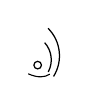
\begin{tikzpicture}[scale=.48,baseline=-1pt]
\draw[line width=.45pt] (0,0) circle (.10);
\draw[line width=.45pt] (.28,-.18) arc (-28:42:.68);
\draw[line width=.45pt] (.42,-.30) arc (-32:45:1.03);
\draw[line width=.40pt] (-.25,-.23) .. controls (0,-.34) and (.18,-.33) .. (.32,-.24);
\end{tikzpicture}
\end{flushright}
\end{document}
